 %!TEX root=title.tex
\label{apndx_usecases}
 %!TEX root=title.tex
\section{Use Cases}
This part will list the properly formulated use cases that can be derived from the gathered requirements.

\subsection{Akteure}
\begin{itemize}
\item User \\ 
Common user who uses the plugin to use Social Weaver.

\item Plugin \\ 
In context of the thesis the Firefox plugin mentioned in section \ref{sowe-firefox} \nameref{sowe-firefox}.

\item Server Service \\ 
\end{itemize}

\subsection{Use Cases}

\subsubsection[Web Element Marking]{User can mark a web element for annotation}
\begin{tabular}{|l| p{6cm} |}
\hline 
 \multicolumn{2}{|c|}{\textbf{Use Case}} \\ 
 \multicolumn{2}{|c|}{User can mark web element for annotation} \\ 
\hline 
Use Case Description & User should be able to see what elements in the web view are annotable. In case his cursor moves above a annotatable element it should be visually marked. \\ 
\hline 
Initiator & User who is performing an interface action. \\ 
\hline 
Pre Condition & User needs to see what web elements are ready to be marked.\\ 
\hline 
Process & Starting position is that the users sees some kind of web view with the plugin activated. Then the user enables the mode in which web elements are highlighted, that might be marked. From here it becomes possible to mark an element by simply clicking it. This brings the plugin into a new state where the type of an annotation can be specified. \\ 
\hline 
After Condition & A successful marking is the precondition for an annotation action. \\ 
Miscellaneous &  \\ 
\hline 
\end{tabular} 

\subsubsection[Web Element Annotating]{User can annotate a web element}
\begin{tabular}{|l| p{6cm} |}
\hline 
 \multicolumn{2}{|c|}{\textbf{Use Case }} \\ 
 \multicolumn{2}{|c|}{User can annotate a web element} \\ 
\hline 
Use Case Description & User should be able to annotate a specific web element so that we can use it as anchor in the future. \\ 
\hline 
Initiator & User who is performing an interface action. \\ 
\hline 
Pre Condition & UseC A. is the precondition for this Use Case. \\ 
\hline 
Process & After the user marked an web element, the next step is to define the type of the annotation. What types are available depends on the state of the plugin or modifications. At this point we just assume an annotation were created and attached to the web element. From here the next condition is to make this annotation visible to the user who is author - or other users who just have a reader role. \\ 
\hline 
After Condition & A successful annotation is the precondition for a visualization of an annotation object. \\ 
\hline 
Miscellaneous &  \\ 
\hline 
\end{tabular} 

\subsubsection[Displaying Annotations]{Plugin can display annotated elements}
\begin{tabular}{|l| p{6cm} |}
\hline 
 \multicolumn{2}{|c|}{\textbf{Use Case}} \\ 
 \multicolumn{2}{|c|}{Plugin can display annotated elements} \\ 
\hline 
Use Case Description & Already annotated web elements in a view should be recognized by the plugin and signals shown to the user where to find which annotations. \\ 
\hline 
Initiator & Indirectly by a user who opens a view, which triggers the matching process of the plugin. \\ 
\hline 
Pre Condition & Already existing annotated elements that might be displayed.  \\ 
\hline 
Process & At this stage we assume an annotation was created. It is not relevant whether the current user is the author of the annotation or a just random user. She opens a web view were an annotation is available. The web element that serves as anchor that is visually highlighted. Further interaction with it lead to an extended view that allows the current user to observe or interact with the annotation. \\ 
\hline 
After Condition & \\ 
\hline 
Miscellaneous & \\ 
\hline 
\end{tabular} 

\subsubsection[Client: Sending Annotations]{Plugin can send Annotations to Server}
\begin{tabular}{|l| p{6cm} |}
\hline 
 \multicolumn{2}{|c|}{\textbf{Use Case }} \\ 
 \multicolumn{2}{|c|}{Plugin can send Annotations to Server} \\ 
\hline 
Use Case Description & The plugin sending data about annotations to the server is one part that is necessary to provide synchronization between user sessions. \\ 
\hline 
Initiator & Social Weaver Plugin Instance \\ 
\hline 
Pre Condition & An annotation has been created \\ 
\hline 
Process & After a user created a new annotation, this issue needs to be updated at the web service. It is necessary that the plugin is able to pack up the information about the way how the annotation is anchored to the web element and about the annotation itself. This package is to be transmitted to the web service where it is processed and stored. \\ 
\hline 
After Condition &  \\ 
\hline 
Miscellaneous &  \\ 
\hline 
\end{tabular} 

\subsubsection[Client: Receiving Annotations]{Plugin can retrieve Annotations from Server Service}
\begin{tabular}{|l| p{6cm} |}
\hline 
 \multicolumn{2}{|c|}{\textbf{Use Case }} \\ 
 \multicolumn{2}{|c|}{Plugin can retrieve Annotations from Server Service} \\ 
\hline 
Use Case Description & Annotations created by other users or in previous sessions are stored at the server. This information needs to be synchronized with the plugin.\\ 
\hline 
Initiator & Plugin and partially Web Service. This means the update might be initiated by the plugin by simply requesting it. On the other hand the update procedure itself is performed by the web service. \\ 
\hline 
Pre Condition & Existing and synchronized annotations at the server. \\ 
\hline 
Process & The process starts when a plugin requests an update from the web service. The origin for that can either be a default update at plugin start up or after an annotation is created and sent to the server. Either way, after the request is sent, the plugin keeps listening for the update messages. The messages needs to be in a format (analogous to the sending use case) that can be parsed to relevant information about annotation location and the type. \\ 
\hline 
After Condition & \\ 
\hline 
Miscellaneous & \\ 
\hline 
\end{tabular} 


\subsubsection[Server: Sending Annotations]{Server Service can send Annotations Updates to Plugin}
\begin{tabular}{|l| p{5cm} |}
\hline 
 \multicolumn{2}{|c|}{\textbf{Use Case }}\\
 \multicolumn{2}{|c|}{Server Service can send Annotations Updates to Plugin}\\ 
\hline 
Use Case Description & Data that is persisted at the server needs to be transmitted to clients in a according format.\\ 
\hline 
Initiator & Web Service. Even though the request may come from the client; the actual procedure is triggered at the back end. \\ 
\hline
Pre Condition & Already persisted annotations in server database. \\ 
\hline 
Process & Once the web service receives the request to send update messages, this happens in a context of a specific URL and an update time stamp. According to those parameters a query is created. The retrieved data is parsed into a format that is readable by the client and transmitted. \\ 
\hline 
After Condition & \\ 
\hline 
Miscellaneous & This use case does not consider knowledge about different users. This means that a single server session provides a synchronous view for all users. \\ 
\hline 
\end{tabular} 

\subsubsection[Server: Receiving Annotations]{Server Service can retrieve Annotations from Plugin}
\begin{tabular}{|l| p{5cm} |}
\hline 
 \multicolumn{2}{|c|}{\textbf{Use Case }} \\ 
 \multicolumn{2}{|c|}{Server Service can retrieve Annotations from Plugin} \\ 
\hline 
Use Case Description &  This use case is the successor for the sending procedure that takes place at the plugin.\\ 
\hline 
Initiator & Plugin \\ 
\hline 
Pre Condition & Successful sending operation from client \\ 
\hline 
Process & Assuming the web service receives some kind of JSON message, it needs to be able to parse it and process it. The payload and url needs to be distinguished and persisted. Persisting can either mean that a new entity ist created or updated. In both cases a fresh time stamp is added before the final persistance operation. \\ 
\hline 
After Condition & \\ 
\hline 
Miscellaneous & Security measures are definitey needed, since otherwise any RESTful request would be processed without validating its origin. \\ 
\hline 
\end{tabular} 


\newpage
\section{Google Calendar Scenario - Screenshot  Walkthrough}
This section repeats the steps for the scenario in Section \ref{web2-scenario}, showing every step as a screenshot. 

\begin{figure}[!h]\centering
		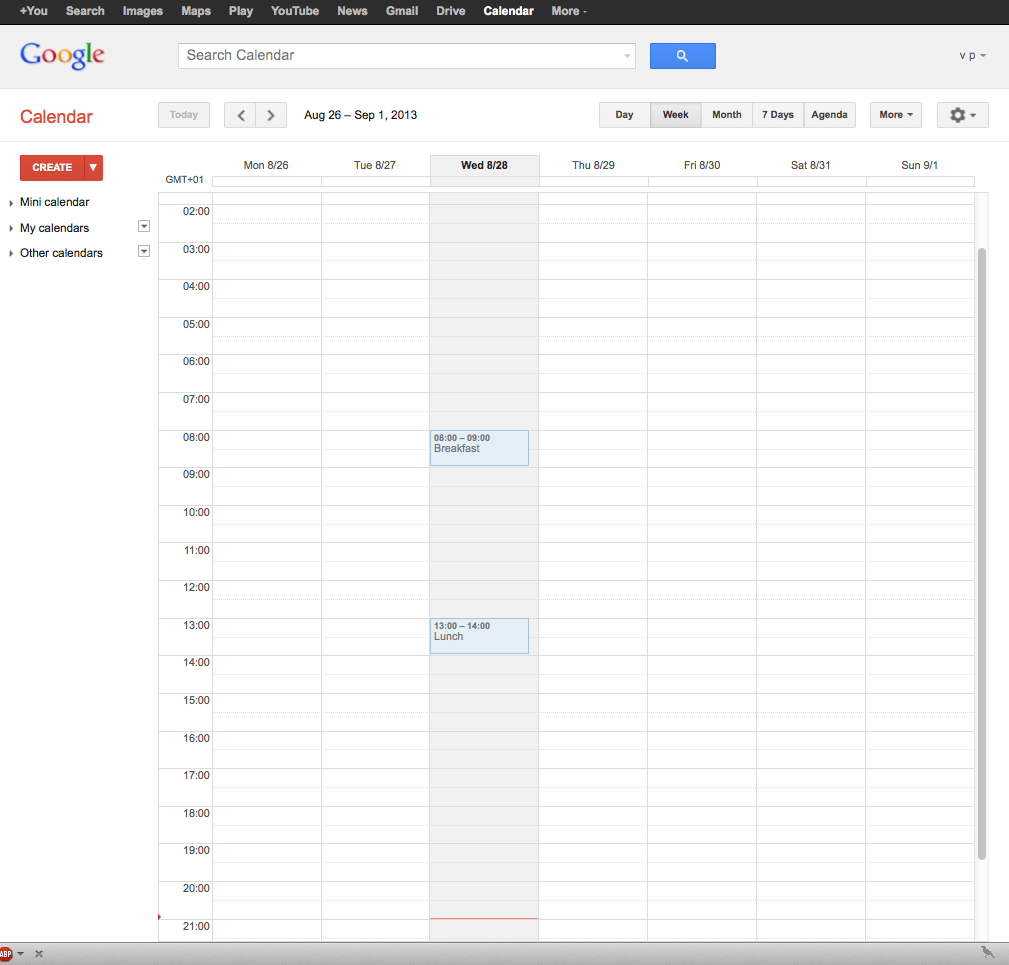
\includegraphics[width=13cm]{images/gcal-screenshot-walkthrough/gcal-wt-1.png}
		\caption{Step 1: GCal is open and the Social Weaver plugin is installed.}
		\label{gcal-wt-1}
\end{figure} 

\begin{figure}\centering
		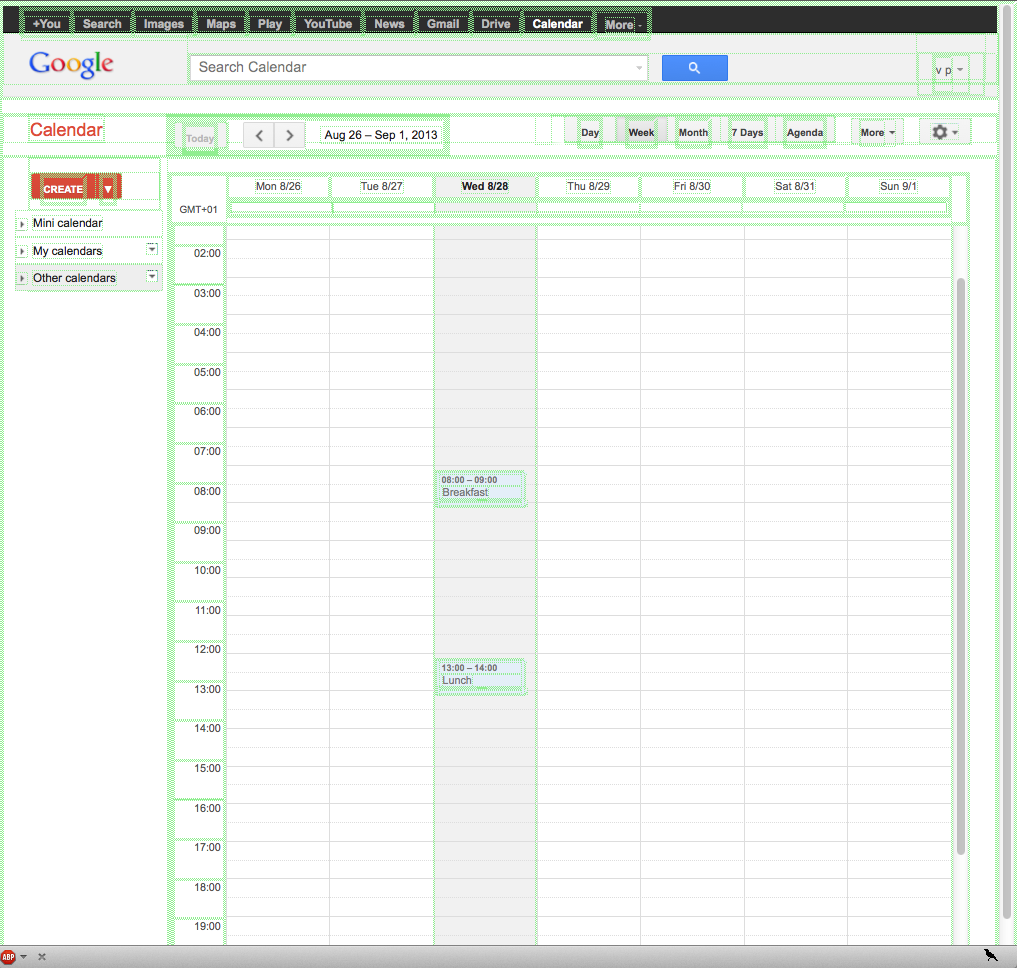
\includegraphics[width=13cm]{images/gcal-screenshot-walkthrough/gcal-wt-2.png}
		\caption{Step 2: The selection mode is activated and all elements are highlighted, which might be selected.}
		\label{gcal-wt-2}
\end{figure} 

\begin{figure}\centering
		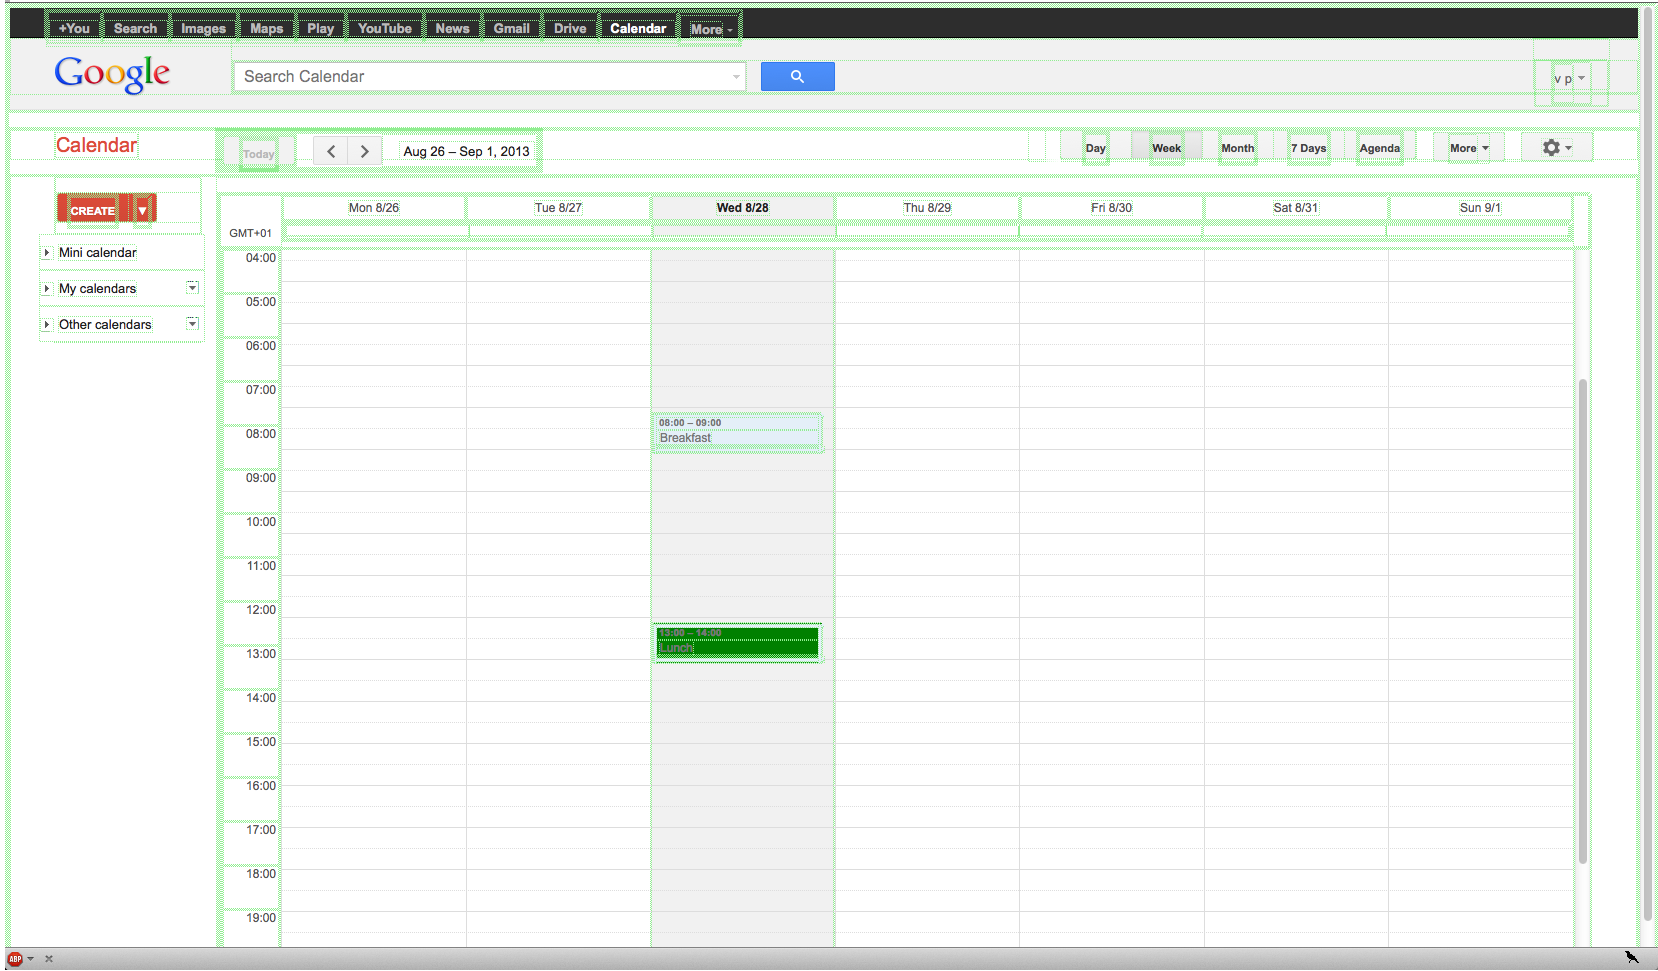
\includegraphics[width=13cm]{images/gcal-screenshot-walkthrough/gcal-wt-3.png}
		\caption{Step 3: The cursor is above the second appointment, therefore it is highlighted in green.}
		\label{gcal-wt-3}
\end{figure} 

\begin{figure}\centering
		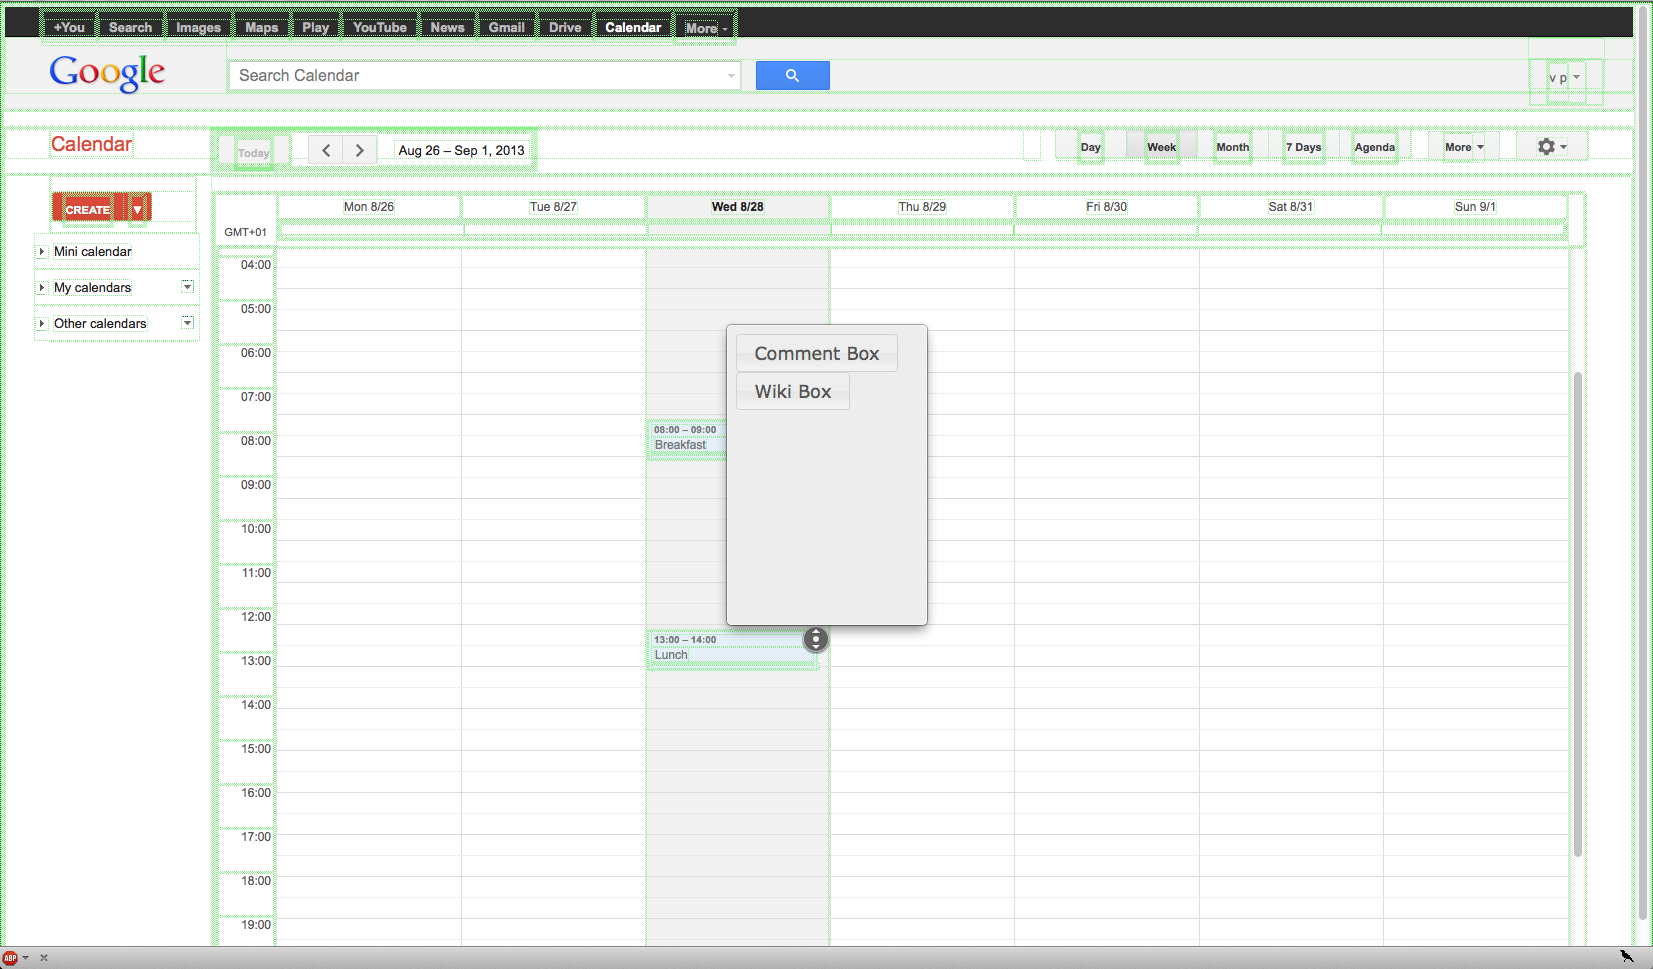
\includegraphics[width=13cm]{images/gcal-screenshot-walkthrough/gcal-wt-4.png}
		\caption{Step 4: The appointment has been clicked, so the annotation-selection procedure becomes visible.}
		\label{gcal-wt-4}
\end{figure} 

\begin{figure}\centering
		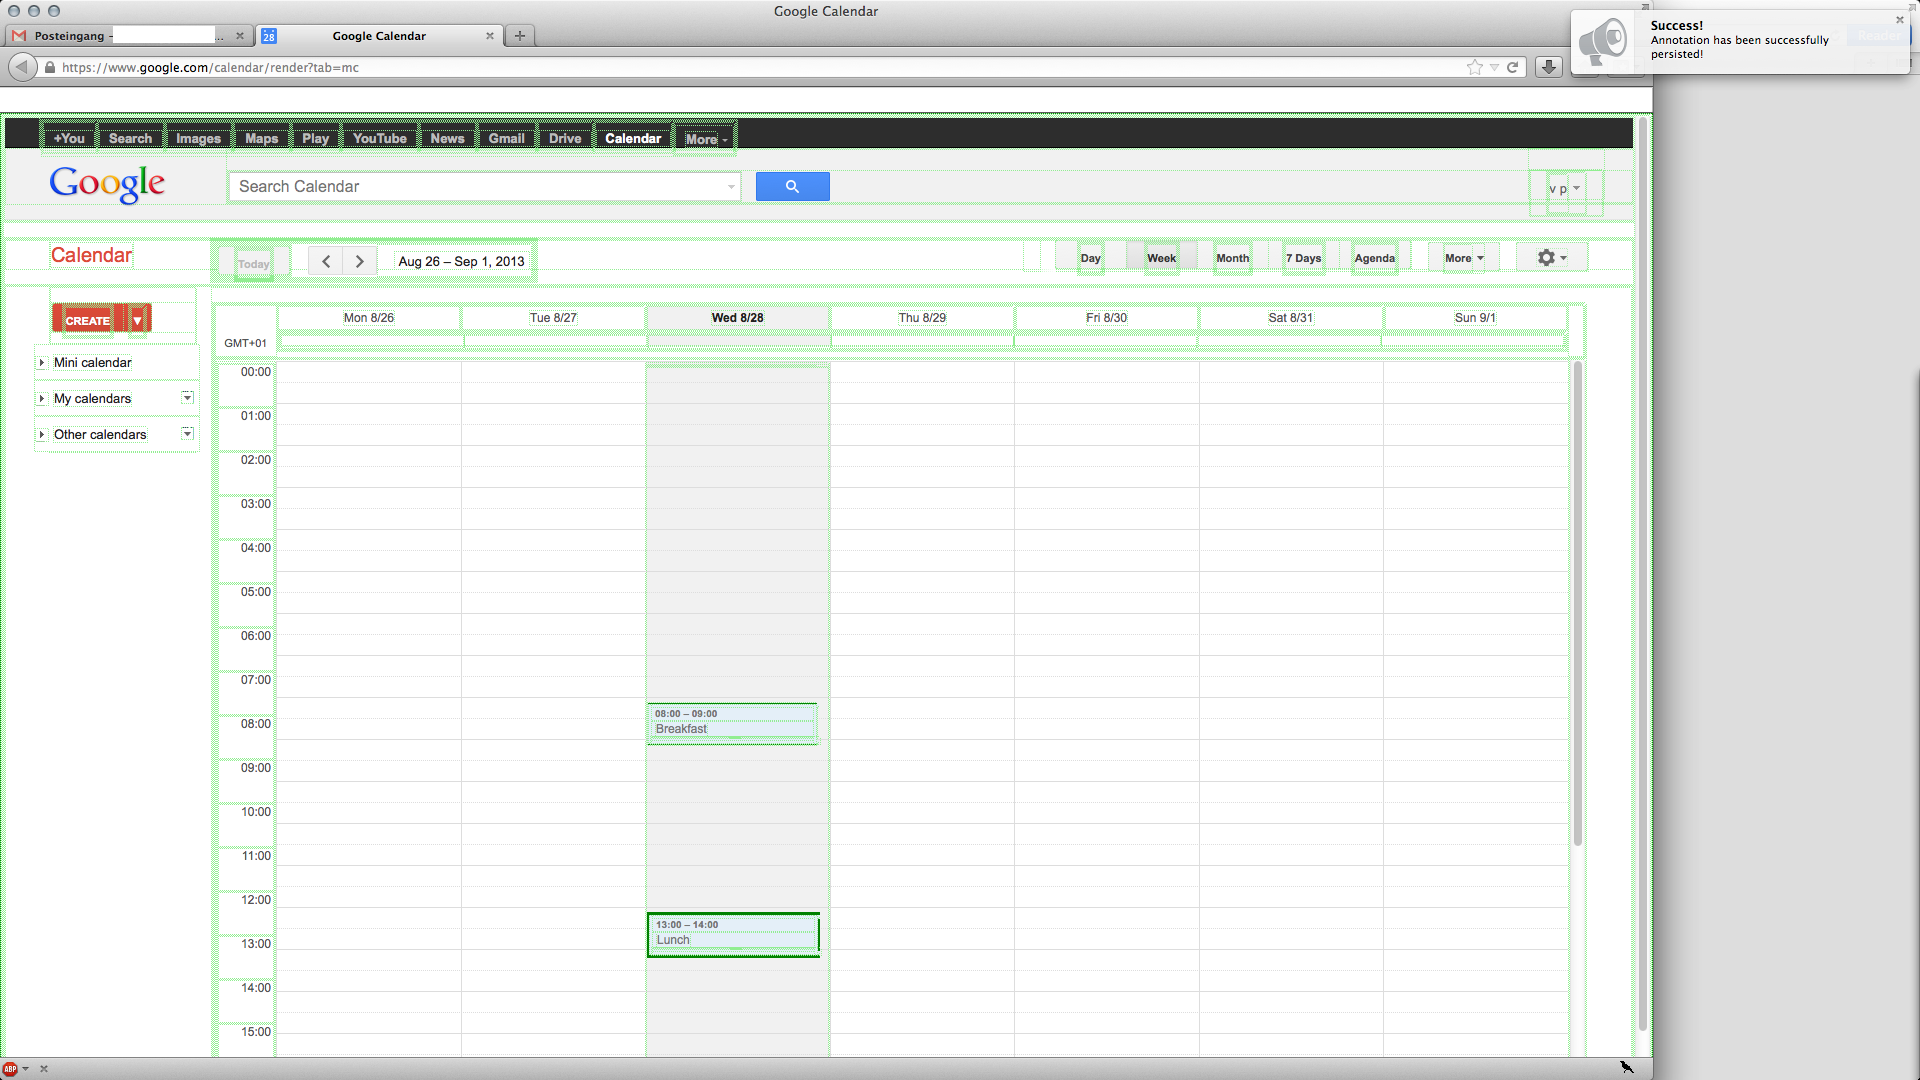
\includegraphics[width=13cm]{images/gcal-screenshot-walkthrough/gcal-wt-5.png}
		\caption{Step 5: The message in the upper-right corner shows that an annotation is persisted successfully.}
		\label{gcal-wt-5}
\end{figure} 

\begin{figure}\centering
		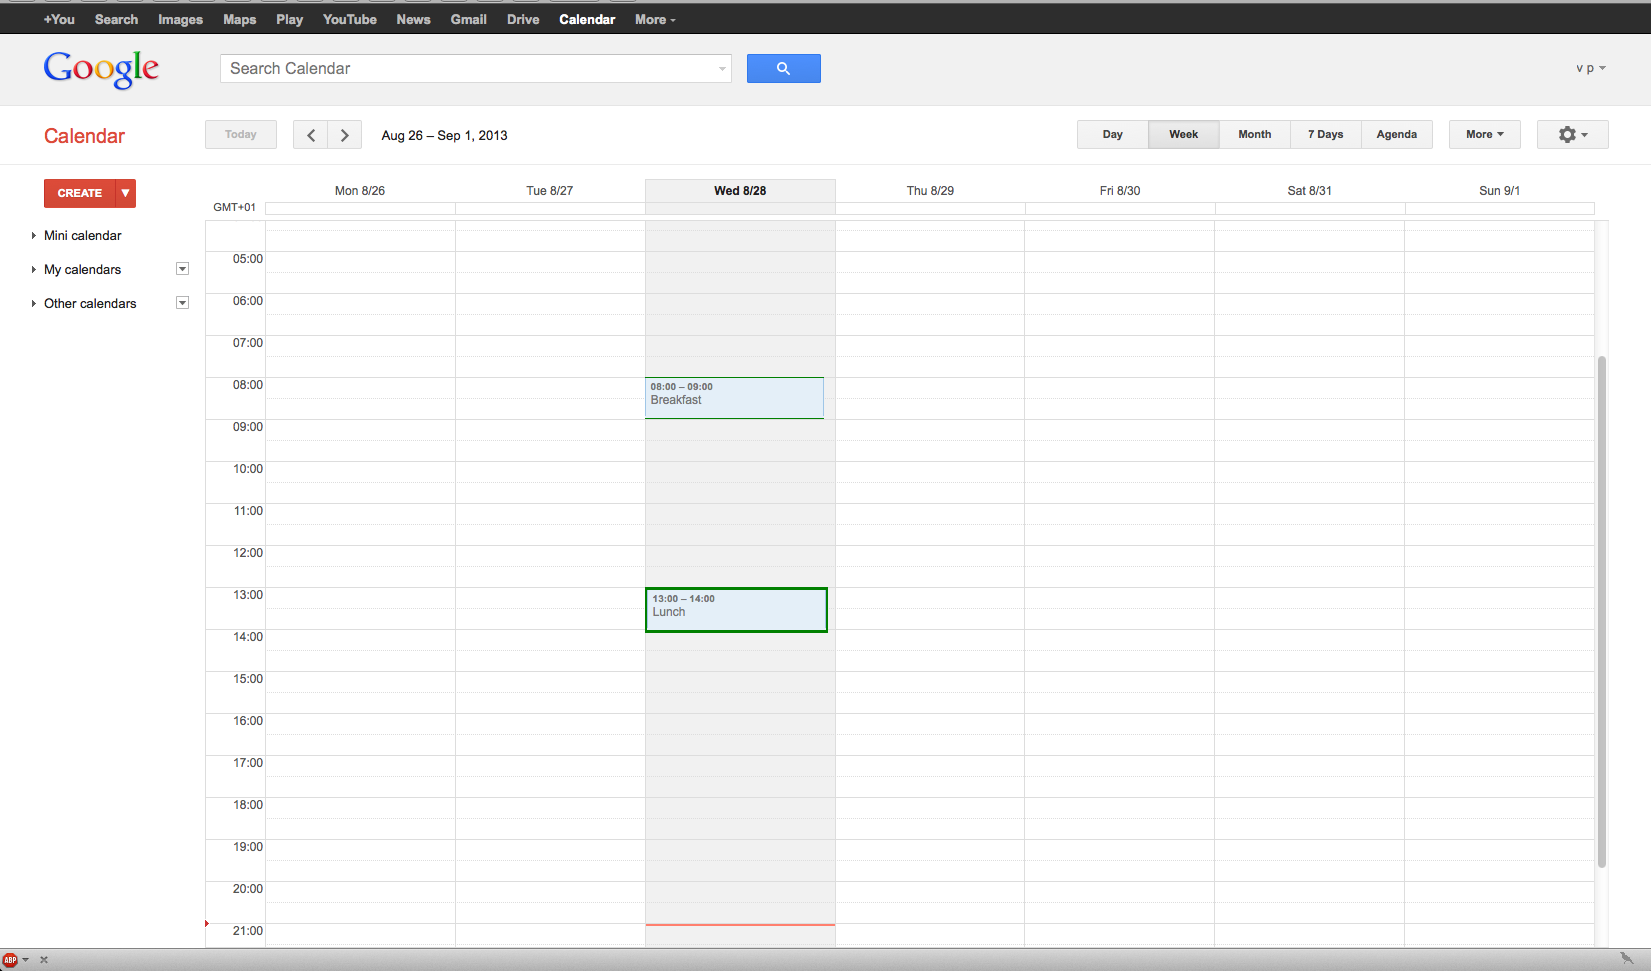
\includegraphics[width=13cm]{images/gcal-screenshot-walkthrough/gcal-wt-6.png}
		\caption{Step 6: After deactivating the selection mode, the annotated element appears inside a green rectangle.}
		\label{gcal-wt-6}
\end{figure} 

\begin{figure}\centering
		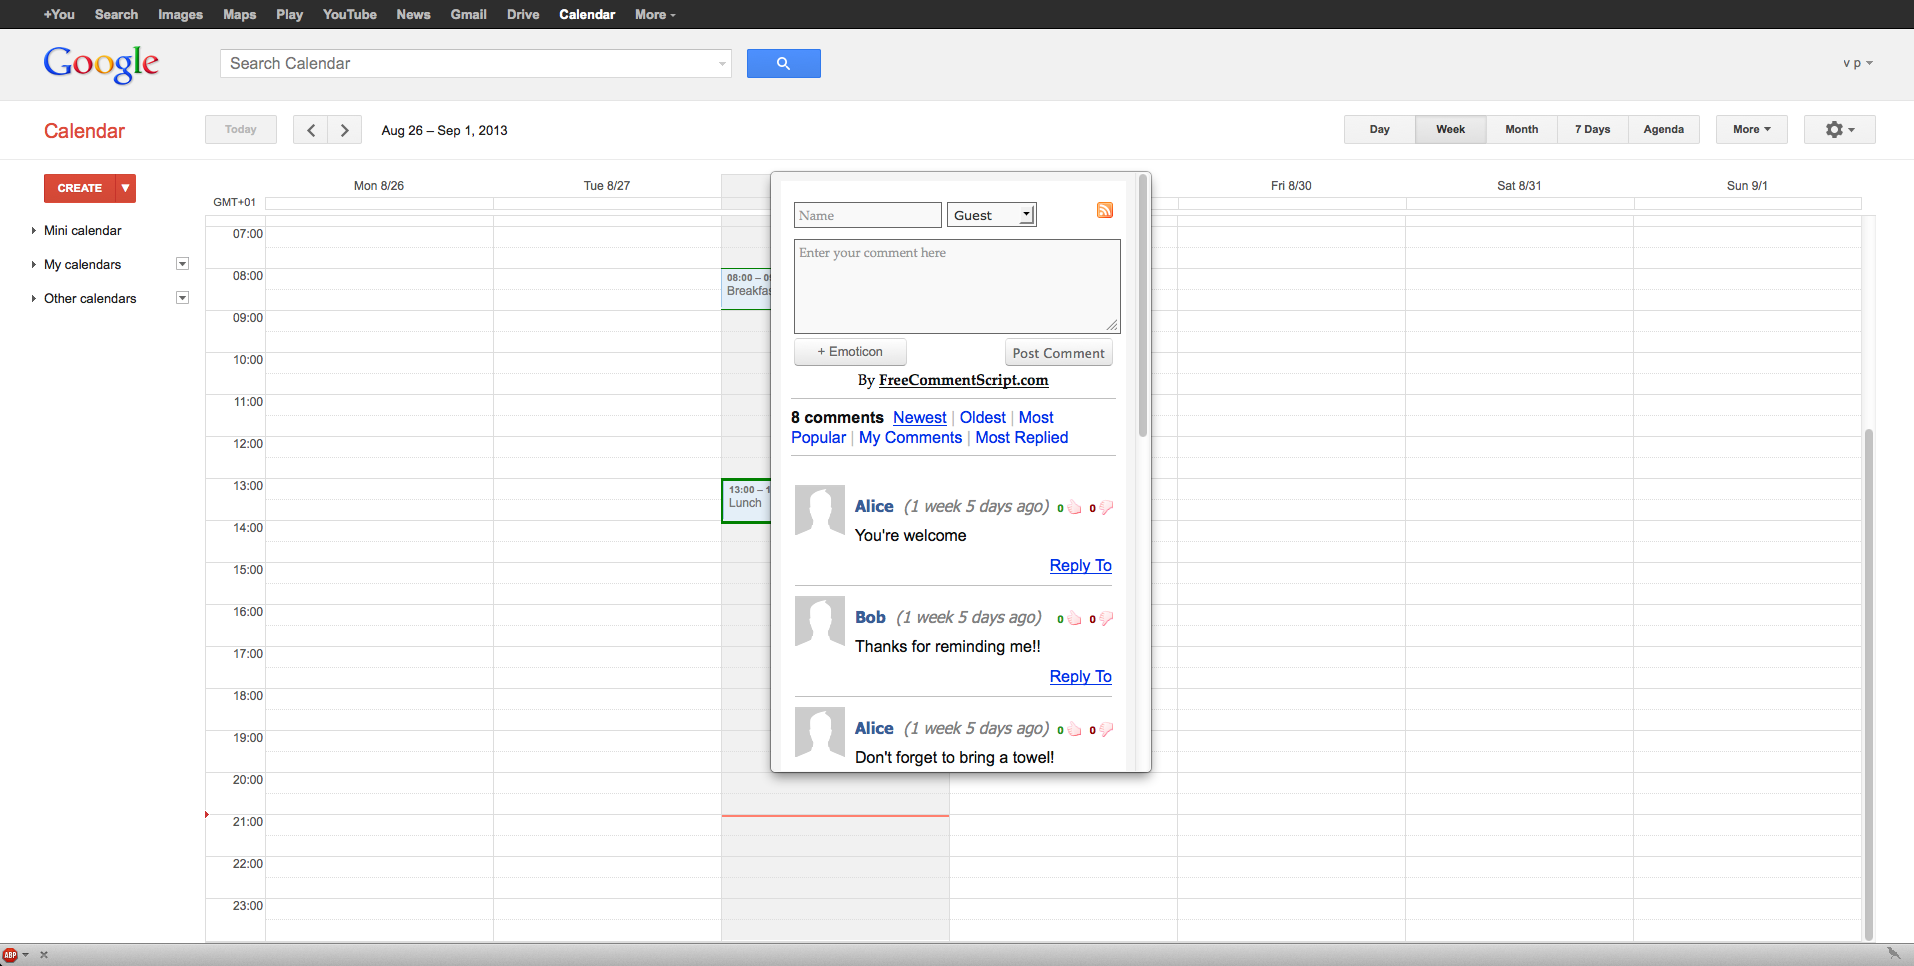
\includegraphics[width=13cm]{images/gcal-screenshot-walkthrough/gcal-wt-7.png}
		\caption{Step 7: A click on the rectangle, open the weaved-in annotation.}
		\label{gcal-wt-7}
\end{figure} 